\appendix
\section*{Appendix}

\section{Overview of migration studies} \label{migration_studies}

The study of migration has been of interest for many areas, such as economics, sociology, geography, demography, and anthropology, among others \citep{cohen_introduction_1996, brettell_introduction_2015}. This characteristic makes migration studies a research field that builds from knowledge and insights from multiple disciplines, and draws on different methods, theories, and definitions \citep{scholten_introduction_2022, brettell_introduction_2015, king_theories_2012}. Ever since the field formally emerged in the late 19th and early 20th centuries, scholars have made an effort to define and structure it in a uniform and cohesive way, but without forgetting its plurality and diversity \citep{scholten_introduction_2022}. This appendix does not aim to address all the nuances of this overly complex field. Instead, it seeks to highlight the main aspects of its development from a historical point of view, to help us contextualize the study of the \textit{economics of migration}, which is an integral part of the field of migration studies. Based on \cite[p. 9-21]{scholten_introduction_2022}\footnote{Their work combines the bibliometric analyses carried out by \cite{levy_between_2020} and \cite{pisarevskaya_mapping_2020}, with ``a strong historical awareness of how the field has developed and how specific topics, concepts, and methods have emerged" \citep[p. 5]{scholten_introduction_2022}.}, we identified that the development of migration studies as a research field can be roughly divided into three periods.

The first period is defined from 1885 until around the 1950s, with the appearance of the first scientific works and the increasing interest of the academic community in the subject. As aforementioned, migration studies as a research field emerged in the late 19th and early 20th centuries, stimulated by rapid urbanization, which was largely caused by rural-urban migration, in industrialized parts of the world, such as the United States (US), the United Kingdom (UK), and Western Europe. The first two works that most likely mark the starting point of the field of migration studies are Raventein's \textit{``The Laws of Migration"} \citep{ravenstein_laws_1885, ravenstein_laws_1889}, considered by many scholars to be the first scientific study on internal migration \citep{scholten_introduction_2022, king_theories_2012, greenwood_early_2003, cohen_introduction_1996}, and Thomas and Znaniecki's work \textit{``The Polish Peasant in Europe and America''}, which is probably the work that started the studies on international migration  \citep{thomas_polish_1927, scholten_introduction_2022}. Nevertheless, most studies in this early period of migration research, like the ones mentioned, lacked formality and adequate techniques. However, it is also true that no appropriate theories or data were available \citep{greenwood_research_1975}.

Among the first disciplines interested in migration research, sociology, demography, and geography stand out. In fact, sociologists, geographers, and demographers had already made important contributions to the field when economists began to take an interest in migration. Economists only began to take a greater interest in migration after the Depression of the 1930s. Coincidentally or not, it was during the 1930s that migration research really picked up, including with the emergence of more formal models. At this moment, migration research was mainly focused on internal migration, especially rural-to-urban movements fuelled by urban growth and urbanization in the so-called developed, or industrialized, countries \citep{greenwood_early_2003}.

The second period happens between around the 1950s and the 1980s, characterized by the field's formalization and expansion. Many important theoretical contributions to the field were made during this period \citep{massey_theories_1993, de_haas_theory_2021}, like Sjaastad's \textit{human capital model} \citep{sjaastad_costs_1962}, Lee’s \textit{theory of migration} \citep{lee_theory_1966}, Harris and Todaro’s \textit{neoclassical migration theory} \citep{todaro_model_1969, harris_migration_1970}, Mabogunje's \textit{migration systems theory} \citep{mabogunje_systems_1970}, and Piore’s \textit{dual labour-market theory} \citep{piore_birds_1979}. As discussed in Section \ref{lit_review_theories}, most of earlier theorisations focused on internal migration, being adapted to analyze international migration later on. In addition, even though the interest in more formal models had already appeared in the 1920s and 1930s, it was only during the 1960s that the field acquired a more formal tone, especially with the use of modified gravity models \citep{greenwood_early_2003}. Regarding the field's expansion, it is reflected by the increase in both the quantity of articles published yearly in migration studies, which jumped from just under 350 in 1975 to almost 750 in 1989 \citep{levy_between_2020, scholten_introduction_2022}, and journals focused on migration and migration-related diversity, which can be seen as the first steps towards the field's institutionalization; according to \cite{pisarevskaya_mapping_2020}, the number of journals grew from zero to 15 in the period between 1959 and 1988. 

Two of the main changes that occurred in this period in relation to the approach to migration studies were: (i) the shift towards a greater focus on international migration, in detriment of internal migration\footnote{For \cite{king_mind_2010}, this shift happened later, during the 1990s and early 2000s.} \citep{scholten_introduction_2022}, driven by the population and economic dynamics of the post-World War II era \citep{castles_migration_2014}, (ii) and a greater attention to issues of ethnic and racial relations involving immigrants, prompted by the civil rights movements in the US in the 1950s and 1960s\footnote{This is just another example of how academically dominant country, or region, such as the US, UK and Europe, have the power to influence, and ultimately dictate, the research agenda.} \citep{portes_immigrant_1978, pedraza-bailey_immigration_1990}; this change was part of a context of greater interest in questions of assimilation and integration of these immigrants in the host societies \citep{scholten_introduction_2022}.

Another important characteristic of the second period is the increase in the number of disciplines interested in migration, which led to the development of the multidisciplinary field as we know it today. However, these disciplines mostly worked in isolation from one another, within their own conceptual frameworks and methodologies \citep{levy_between_2020, scholten_introduction_2022}. Thus, although migration studies was indeed multidisciplinary field by the end of the 1980s, it was definitely not interdisciplinary\footnote{Regarding the concepts of multidisciplinary and interdisciplinary, we follow King's way of thinking, which stated that ``cross- and multidisciplinary implies two or more different disciplines working alongside each other, in parallel so to speak; interdisciplinarity implies a fusing of disciplines in an integrated analysis" \citep[p. 10]{king_theories_2012}.}.

The third and final period in our historical analysis is what \cite{castles_migration_2014} have called the \textit{Age of Migration}, which begins in the 1990s and continues to the present day\footnote{Levy and colleagues seem to indicate a new developmental phase by writing that ``since 2005, a new age of migration studies has emerged" \citep[p. 17]{levy_between_2020}. Therefore, what we are defining as the third period would be broken down in two, one from 1990 to 2005, and the other from 2005 to the present. In any case, we decided to stick to our initial division.}, during which migration has become more diverse, globalized, politicized, and feminized\footnote{\cite{castles_migration_2014} actually point out to the fact that women have played an increasing role in labor migration since the 1960s, which falls into our second period. In any case, after 1990s, women started forming the majority in multiple movements of workers.} \citep{king_theories_2012, castles_migration_2014}. The defining characteristic of the \textit{Age of Migration} is the political prominence of the topic of migration\footnote{As stated by \cite{king_mind_2010}, during this time migration came to be understood as international migration. For Scholten and colleagues, this was due to ``a move beyond a strong focus on the national dimension of migration and diversities" \citep[p. 16]{scholten_introduction_2022}.}. As Castles and colleagues have stated, what is distinctive in recent migratory movements ``is their global scope, their centrality to domestic and international politics and their considerable economic and social consequences" \citep[p. 6]{castles_migration_2014}. The unprecedented speed of communications and transportation--combined with the social, economic, and political transformations that the world underwent after the end of the Cold War--haa intensified globalization impulses, and, consequently, the movement of people across borders. In this context, politicians and policy-makers have seen this phenomenon as a threat to the sovereignty of states and their ability to regulate and control immigrant flows, which has contributed to the rise of anti-immigration sentiment \citep{martiniello_introduction_2012, castles_migration_2014}.

Regarding the scientific production in the third period, the field has seen a notable acceleration. If the number of migration studies published in 1989 had been slightly under 750, this number increased to 1,000 in 1995, and reached the remarkable figure of 3,000 in 2017 \citep{levy_between_2020, scholten_introduction_2022}. A noteworthy methodological change in the field since the early 1990s, noted by \cite{king_theories_2012}, was the shift from quantitative to qualitative research, which was influenced by new approaches, insights, and perspectives arising mainly from qualitative sociology, anthropology, human geography, and cultural studies. This shift reflected the widespread moment in the social sciences that King called ``cultural turn", which, according to him, ``did not so much re-make theories of the causes of migration as enrich our understanding of the migrant experience" \citep[p. 25]{king_theories_2012}. As pointed out by \cite{scholten_introduction_2022}, this meant that migration studies were shifting from migration to migrants, that is, there was an increase in the importance of ``research on the subjective experiences of migrants, perceptions of migrants’ identity and belonging, as well as attention to the cultural (super)diversity of societies" \citep[p. 21]{scholten_introduction_2022}.

According to King, ``the `Age of Migration' has seen a proliferation of new types of migration and international mobility which form important elements of the increasingly complex global map of population movements" \citep[p. 9]{king_theories_2012}], such as \textit{transnationalism} \citep{schiller_transnationalism_1992} and \textit{diasporas} \citep{cohen_global_2008}, which were added to the conceptual frameworks of migration studies \citep{king_theories_2012}. The typological discussion of these types of migration and migrants has been a source of controversy because some definitions involve complications related to the way migration unfolds in time and space, and also because of many conceptual differences found in the social sciences\footnote{For a more detailed discussion, see \cite{king_theories_2012}, p. 7-9.}. In the end, all these differences between the social sciences in their approach to migration studies were viewed as a major barrier, as eloquently expressed by Massey and colleagues:

\begin{quote}
Social scientists do not approach the study of immigration from a shared paradigm, but from a variety of competing theoretical viewpoints fragmented across disciplines, regions, and ideologies. As a result, research on the subject tends to be narrow, often inefficient, and characterized by duplication, miscommunication, reinvention, and bickering about fundamentals and terminology \citep[p. 700-701]{massey_evaluation_1994}.
\end{quote}

In light of this problem, some authors called for more integration between disciplines. \cite{king_towards_2002} and \cite{king_theories_2012} called for an ``interdisciplinary synthesis", while \cite{brettell_introduction_2015} proposed a ``talk across disciplines" in an effort to bring them closer together. Moving away from the sphere of mere rhetoric, important contributions were made to seek a convergence in terminology. For instance, Cohen presented his nine \textit{dyads}\footnote{Also called dichotomies or binaries \citep{king_theories_2012}.}, which, according to him, were ``building blocks to a theory of migration" \citep[p. xvi]{cohen_introduction_1996}. \cite{king_towards_2002} called for a deconstruction of the traditional dichotomies presented by Cohen, arguing that migration's motivations and forms have become much more diverse. The author offered new geographies and typologies of (international) migration applied to the European context, while stressing the need for a more integrated approach that ``brings together and integrates a range of perspectives, frameworks, theoretical stances and methodologies in order to study migration (or the various forms of migration)" \citep[p. 90]{king_towards_2002}.

However, some studies provide quantitative evidence that migration studies may have been more interdisciplinary than perceived. The investigation into the field's topical composition performed by \cite{pisarevskaya_mapping_2020} showed that, overall, the field's topics have been well-connected at least since the late 1980s, which could suggest the existence of a shared conceptual and theoretical language. Another study conducted by Levy, Pisarevskaya, and Scholten found a growing coherence between the epistemic communities (or co-citation networks), which, according to them, suggests that ``migration studies evolved from a multidisciplinary field (with various but very distinct disciplines) to a more interdisciplinary field (with various and linked disciplines)" \citep[p. 22-23]{levy_between_2020}. In fact, \cite{levy_between_2020} concluded that not only has the field become more interdisciplinary, but it has also increased in terms of internationalization--with a growing number of countries collaborating in the scientific production, even though still in an uneven way--and self-referentiality, which is evidence that the research field of migration studies has institutionalized. Another factor that points to the field's institutionalization is the growing number of journals, which jumped from 15 in 1988 to 45 in 2018, accompanying the accelerated growth in scientific production.

\section{Latent Dirichlet Allocation} \label{LDA}

Latent Dirichlet Allocation (LDA)\footnote{Regarding terminology and notation, we follow \cite{blei_latent_2003}.} builds upon the assumption that documents exhibit multiple topics in different proportions, where a topic is a probabilistic distribution over the words in a fixed vocabulary. The basic unit of an LDA model is a \textit{word}, or \textit{term}, $w$, which is an item from the fixed vocabulary $\{1, \cdots, V \}$; a \textit{document} $\mathbf{w} = (w_{1}, \cdots, w_{n}, \cdots, w_{N})$ is a sequence of $N$ words\footnote{LDA is based on the bag-of-words assumption, according to which words in a document are exchangeable, and so the order of words in a document can be neglected \citep{blei_latent_2003}.}, where $w_{n}$ is the nth word in the sequence; and a \textit{corpus} $D = \{ \mathbf{w}_{1}, \cdots, \mathbf{w}_{m}, \cdots, \mathbf{w}_{M} \}$ is a collection of $M$ documents, where $\mathbf{w}_{m}$ is the mth document in the collection. After the definition of our fixed vocabulary, we shall represent our corpus of $M$ documents as a so-called document-term matrix (DTM)\footnote{Representing our corpus as a DTM is only possible under the bag-of-words assumption \citep{ponweiser_latent_2012}.}, as shown in Table \ref{tab:dtm}.

\begin{table}[ht!]
	\centering
	\begin{tabular}{c|cccccc}
           		        & Word 1 ($w_{1}$) & Word 2 ($w_{2}$) & $\cdots$ & Word $n$ ($w_{n}$) & $\cdots$ & Word $V$ ($w_{V}$) \\ \hline
Document 1 ($\mathbf{w}_{1}$) & 1 & 2 & $\cdots$ & 4 & $\cdots$ & 0 \\
Document 2 ($\mathbf{w}_{2}$) & 0 & 4 & $\cdots$ & 3 & $\cdots$ & 0 \\
$\vdots$ & $\vdots$ & $\vdots$ & $\vdots$ & $\vdots$ & $\vdots$ & $\vdots$ \\
Document $m$ ($\mathbf{w}_{m}$) & 2 & 2 & $\cdots$ & 0 & $\cdots$ & 1 \\
$\vdots$ & $\vdots$ & $\vdots$ & $\vdots$ & $\vdots$ & $\vdots$ & $\vdots$ \\
Document $M$ ($\mathbf{w}_{M}$) & 5 & 0 & $\cdots$ & 1 & $\cdots$ & 2
	\end{tabular}
	\caption{Example of a document-term matrix with $M$ documents and $V$ words, adapted from \cite{ponweiser_latent_2012}. This table represents every document in terms of frequencies of words in our fixed vocabulary. The cells indicate how often a word shows up in a document.}
	\label{tab:dtm}
\end{table}

Other elements of the LDA model are: the number of topics $K = \{ 1, \cdots, k \}$; the parameters $\alpha$ and $\eta$, which follow Dirichlet distributions; $\beta_{k} \sim \text{Dirichlet}(\eta)$, which is defined for a given $\eta$ and indicates the probability of a word occurring given a topic $k$, and follows a Dirichlet distribution; $\theta \sim \text{Dirichlet}(\alpha)$, which is defined for a given $\alpha$ and gives the topic proportions per document $\mathbf{w}_{m}$, and that also follows a Dirichlet distribution; and the topic $z_{n} \sim \text{Mult}(\theta)$, which is a topic assigned for a given $\theta$ and follows a Multinomial distribution \citep{blei_latent_2003, blei_topic_2009, grun_topicmodels_2011}. An illustration of how an LDA model works is presented in Figure \ref{fig:lda}. In a simplified way, LDA applies the following probabilistic generative process \citep{blei_topic_2009, grun_topicmodels_2011, ponweiser_latent_2012}:

\begin{enumerate}
\item For each topic $k$: draw a word distribution $\beta_{k}$;
\item For each document $\mathbf{w}_{m}$ in corpus $D$:
\begin{enumerate}
	\item Draw a topic distribution $\theta$;
	\item For each of the $N$ words $w_{n}$	;
	\begin{enumerate}
		\item Choose a topic $z_{n}$;
		\item Choose a word $w_{n}$ from a multinomial probability $p(w_{n} | z_{n}, \beta_{k})$, conditioned on both the topic $z_{n}$ from step (i) and the word distribution $\beta_{k}$ from step (1).
	\end{enumerate}
\end{enumerate}
\end{enumerate} 

\begin{figure}[!ht]
	\centering
	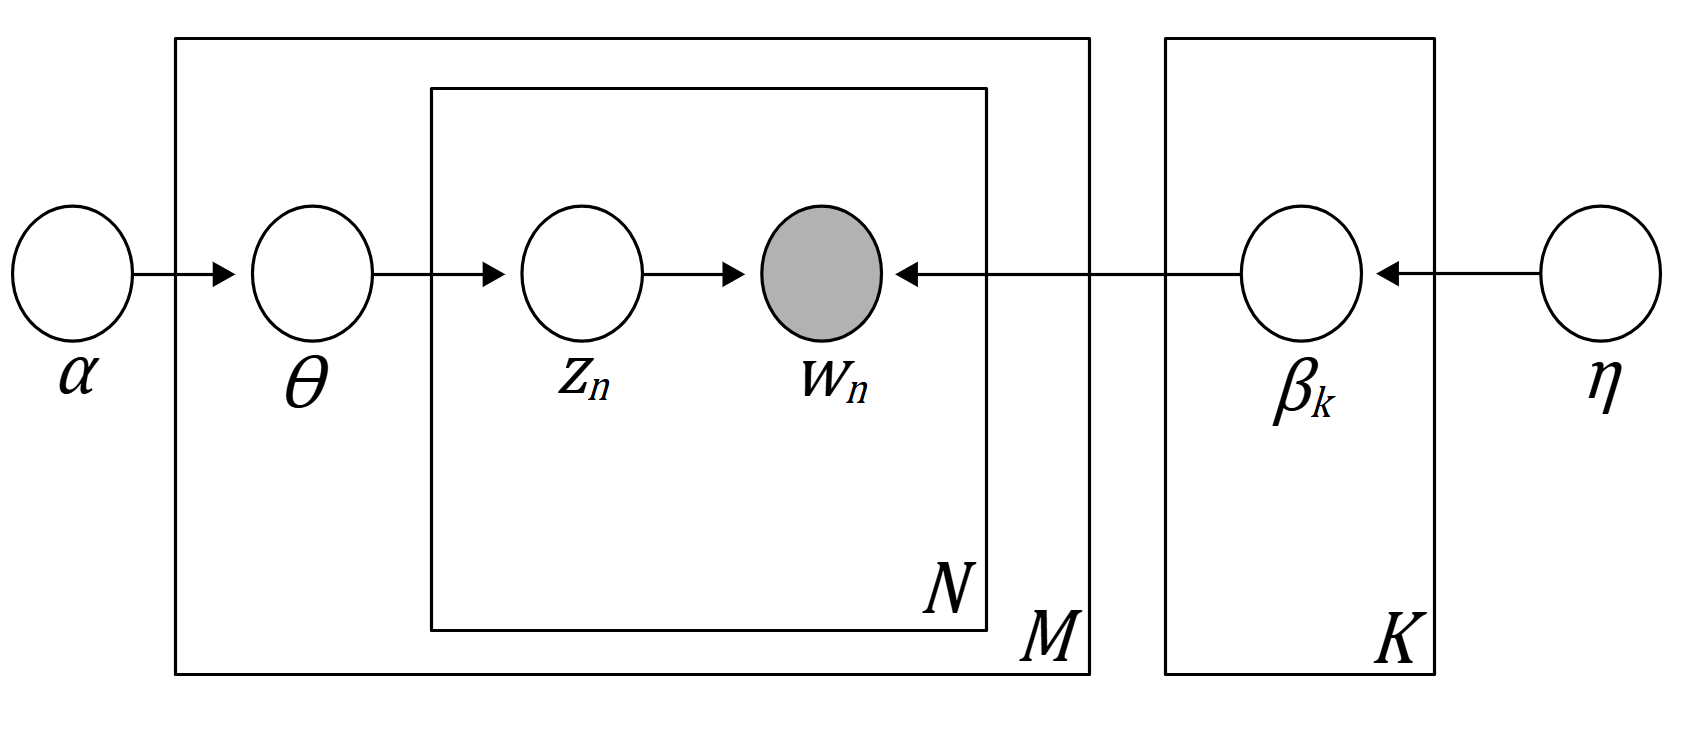
\includegraphics[width=0.6\linewidth]{lda.png}
	\caption{A graphical model representation of LDA, adapted from \cite{blei_latent_2003} and \cite{blei_topic_2009}.}
	\label{fig:lda}
\end{figure}

%\section{Per-topic word probabilities} \label{words_over_topics}
%
%\begin{figure}[!ht]
%	\centering
%	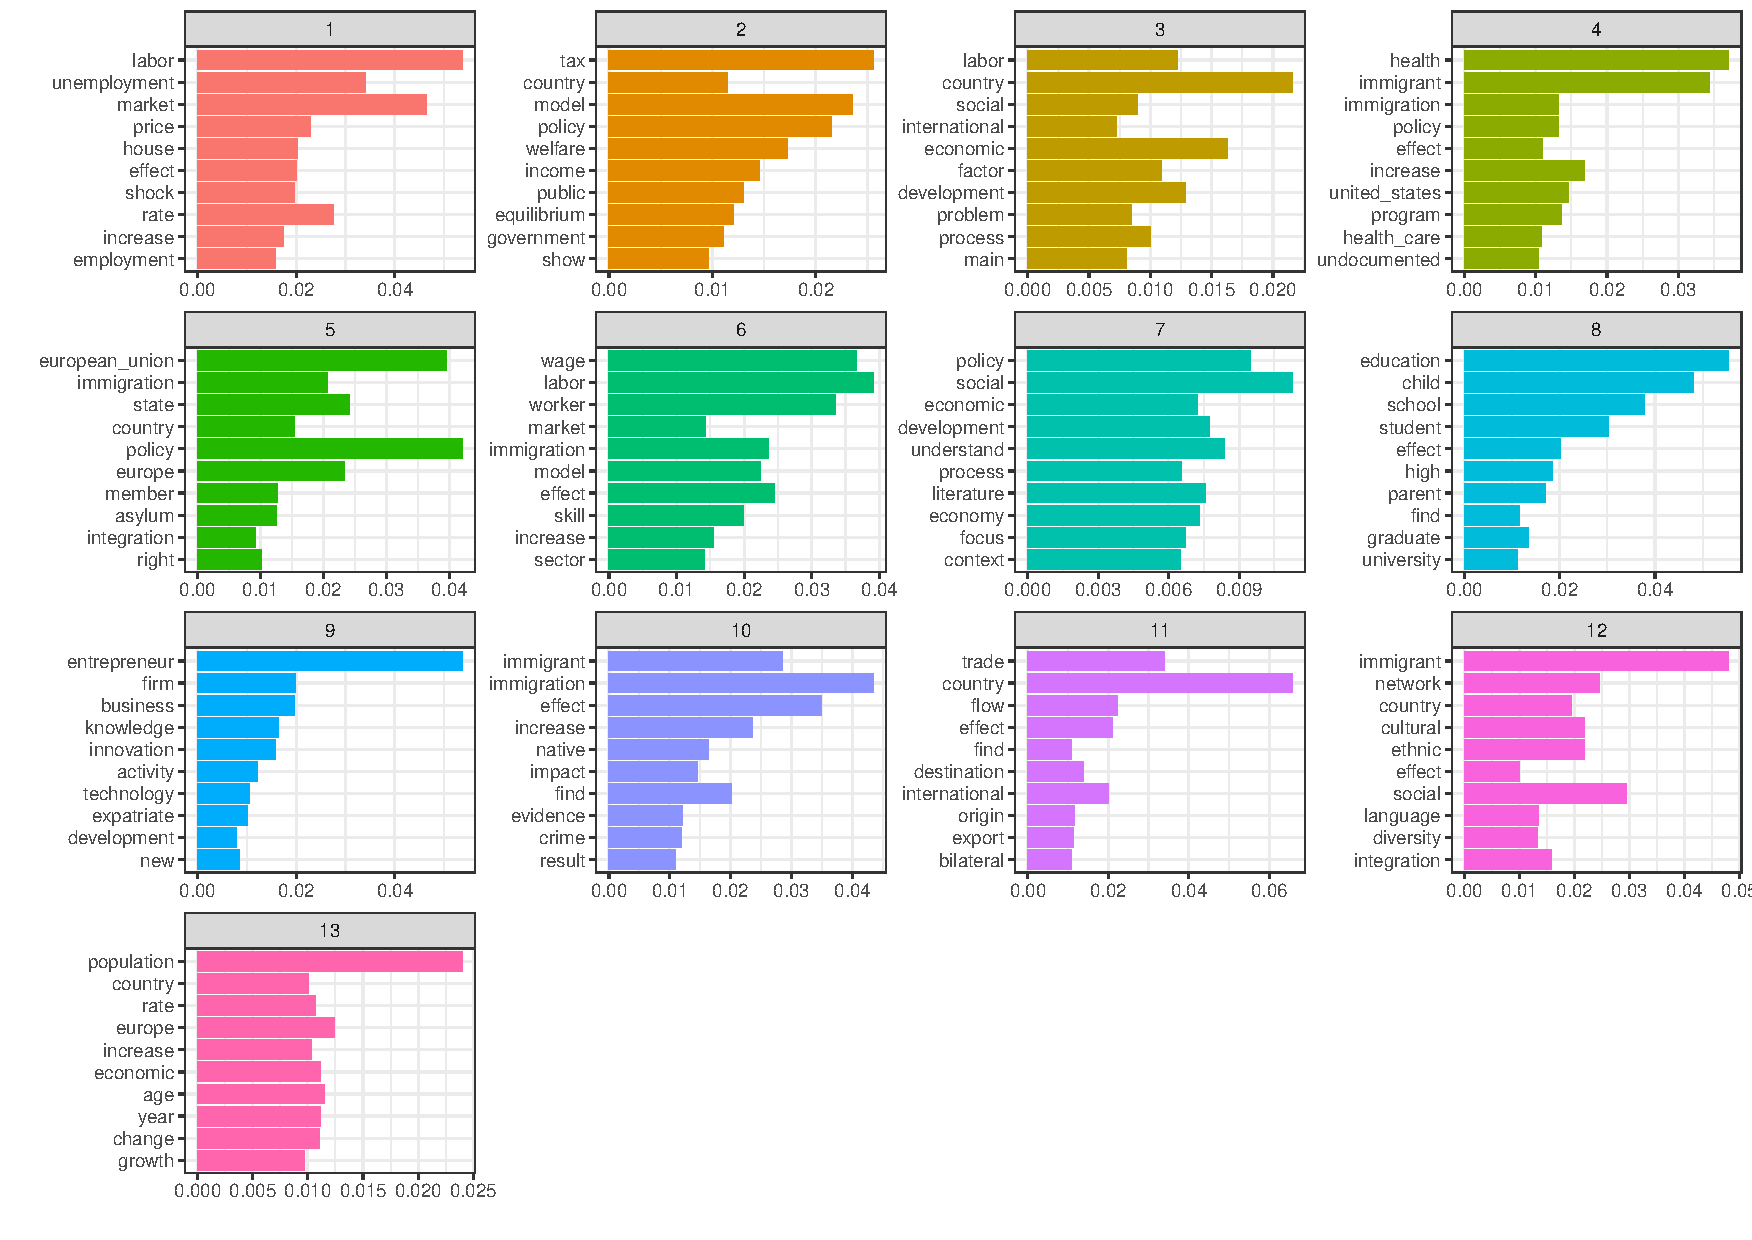
\includegraphics[scale=0.5]{top_terms_figure1.pdf}
%	\caption{Posterior probabilities of words belonging to topics. Ten most likely words over topics 1 to 13.}
%	\label{fig:top_terms_1}
%\end{figure}
%
%\begin{figure}[!ht]
%	\centering
%	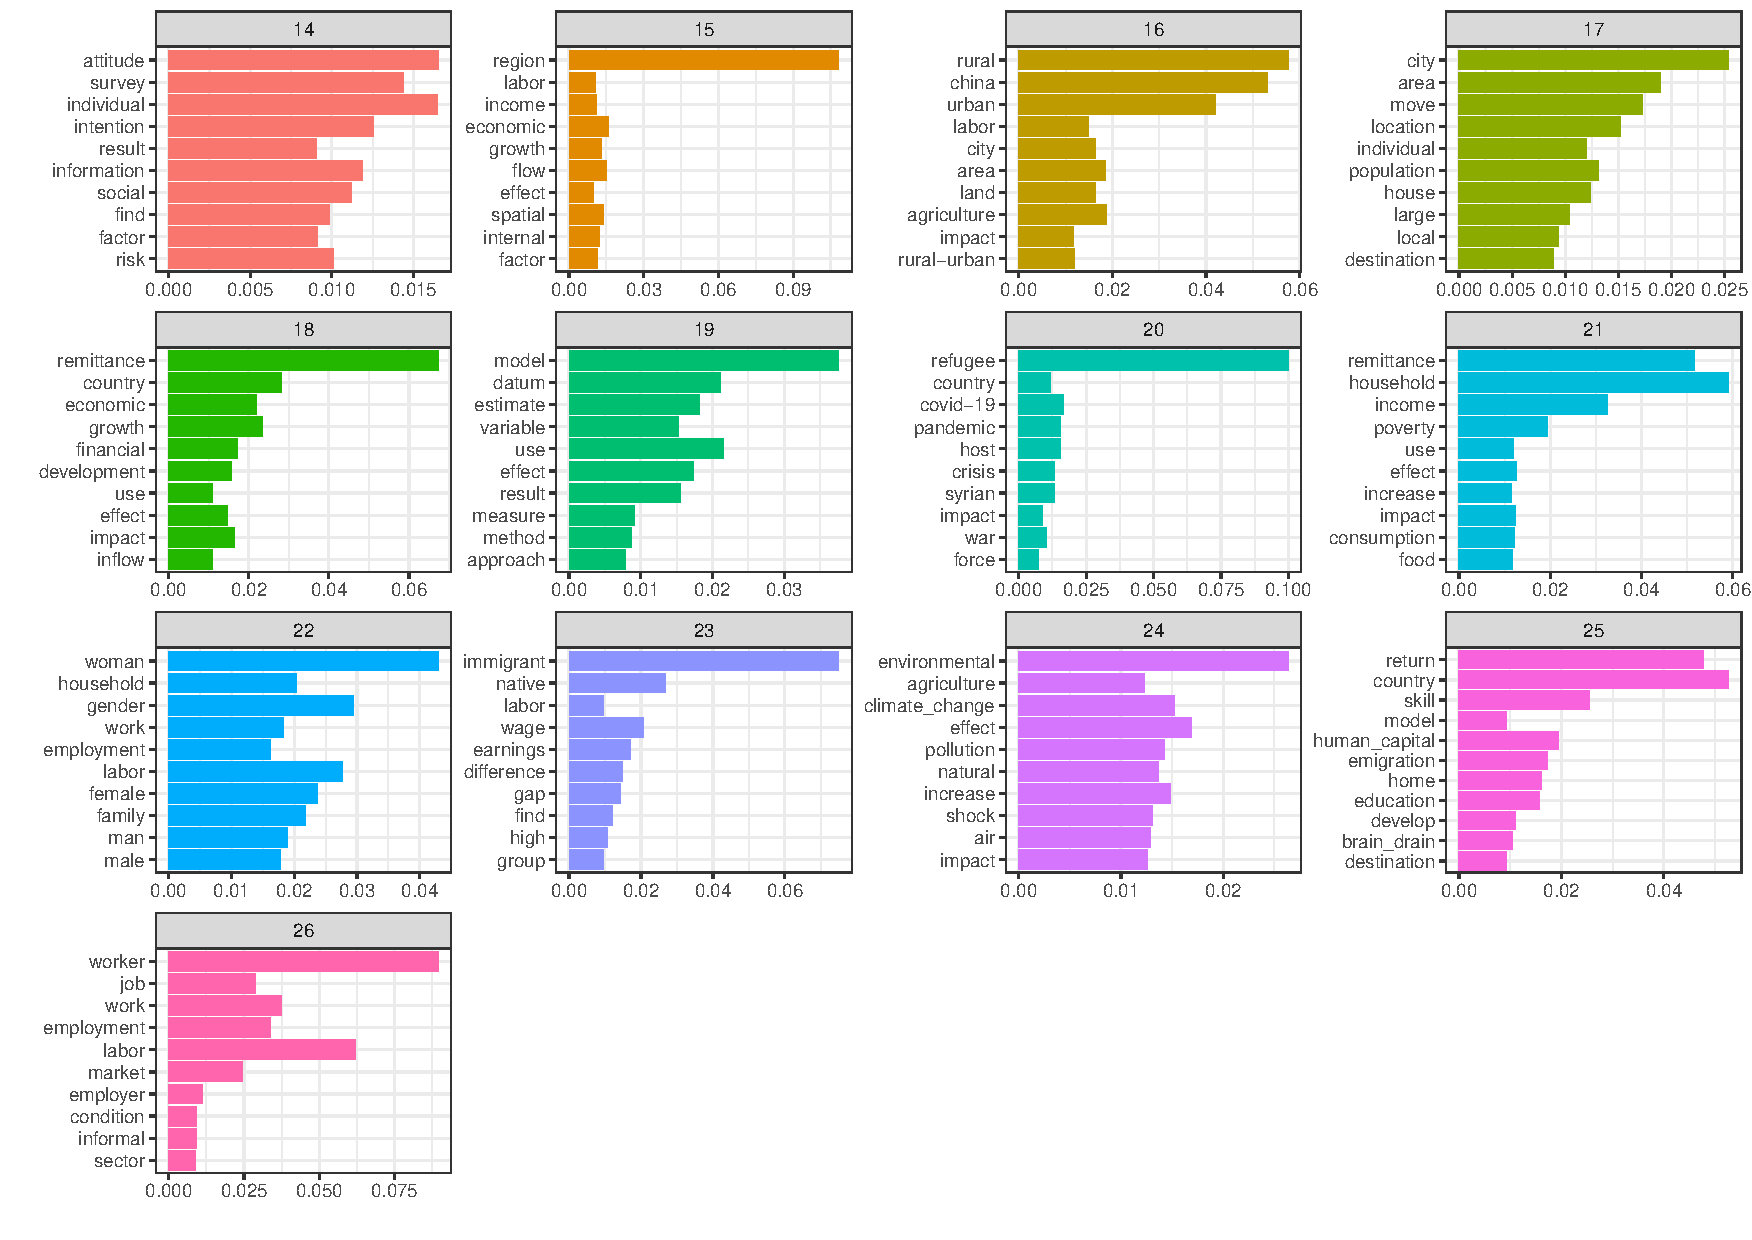
\includegraphics[scale=0.5]{top_terms_figure2.pdf}
%	\caption{Posterior probabilities of words belonging to topics. Ten most likely words over topics 14 to 26.}
%	\label{fig:top_terms_2}
%\end{figure}

\section{The Gini-Simpson and the Shannon-Wiener diversity measures} \label{diversity_indices}

Two of the most famous measures of diversity that have been used in multiple scientific areas are the Gini-Simpson index and the Shannon-Wiener index \citep{jost_entropy_2006}. The Gini-Simpson index was first proposed by \cite{simpson_measurement_1949}, and it can be used to measure the probability of two entities representing different types or species. The formula of the Gini-Simpson index adapted to our study, here referred to as $GS$, is given by:

\begin{equation}
GS = 1 - \sum^{T}_{i = 1} (p_{i})^{2},
\label{gs_entropy}
\end{equation}

\noindent where $T$ is the number of topics, and $p_{i}$ is the topic proportion, with $GS \in [0,1)$. Applied to our case, the index measures the probability that two abstracts of scientific documents selected at random represent different topics. Therefore, the higher the value of $GS$, the more diverse our corpus is because the higher the probability that two documents randomly selected are from different topics.

The Shannon-Wiener index, also called the Shannon entropy, measures uncertainty-related diversity. It was first presented by \cite{shannon_mathematical_1948}, and it measures the uncertainty of identifying an entity at random in a particular group or collection. The index, here referred to as $H$, has the following formula:

\begin{equation}
H = - \sum^{T}_{i = 1} p_{i} \ln{p_{i}},
\label{h_entropy}
\end{equation}

\noindent where $T$ is the number of topics, and $p_{i}$ is the topic proportion, with the value of $H \in [0, \infty)$, where the higher $H$ is, the more diverse our corpus, since we have a greater uncertainty about which topic the document is about when choosing a document randomly in a very diverse collection of documents.

It is worth mentioning that there is a discussion proposed by \cite{jost_entropy_2006}, where the author points out that indices like Gini-Simpson and Shannon-Wiener are actually entropies and not diversities, and follows to propose variations that truly measure diversity. However, Jost also admits that ``entropies are reasonable indices of diversity" \citep[p. 363]{jost_entropy_2006}, leaving it clear that the discussion is much more conceptual. Following this discussion, we decided to present only the indices defined above. In any case, acknowledging the differences, we decided to call our indices \textit{Gini-Simpson entropy index} and \textit{Shannon-Wiener entropy index}.